%% 
%% Copyright 2007, 2008, 2009 Elsevier Ltd
%% 
%% This file is part of the 'Elsarticle Bundle'.
%% ---------------------------------------------
%% 
%% It may be distributed under the conditions of the LaTeX Project Public
%% License, either version 1.2 of this license or (at your option) any
%% later version.  The latest version of this license is in
%%    http://www.latex-project.org/lppl.txt
%% and version 1.2 or later is part of all distributions of LaTeX
%% version 1999/12/01 or later.
%% 
%% The list of all files belonging to the 'Elsarticle Bundle' is
%% given in the file `manifest.txt'.
%% 
%% Template article for Elsevier's document class `elsarticle'
%% with harvard style bibliographic references
%% SP 2008/03/01

%\documentclass[preprint,12pt,authoryear]{elsarticle}  %default in the template
%\documentclass[preprint,10pt,authoryear]{elsarticle}

%% Use the option review to obtain double line spacing
%% \documentclass[authoryear,preprint,review,12pt]{elsarticle}

%% Use the options 1p,twocolumn; 3p; 3p,twocolumn; 5p; or 5p,twocolumn
%% for a journal layout:
%% \documentclass[final,1p,times,authoryear]{elsarticle}
%% \documentclass[final,1p,times,twocolumn,authoryear]{elsarticle}
 \documentclass[final,3p,times,authoryear]{elsarticle}
%% \documentclass[final,3p,times,twocolumn,authoryear]{elsarticle}
%% \documentclass[final,5p,times,authoryear]{elsarticle}
%% \documentclass[final,5p,times,twocolumn,authoryear]{elsarticle}

%% For including figures, graphicx.sty has been loaded in
%% elsarticle.cls. If you prefer to use the old commands
%% please give \usepackage{epsfig}

%% The amssymb package provides various useful mathematical symbols
\usepackage{amssymb}
%% The amsthm package provides extended theorem environments
 \usepackage{amsthm}
 \usepackage{amsmath}
 \usepackage{color}
 \usepackage{amsmath}
\usepackage{siunitx}


\usepackage{framed} % Framing content
\usepackage{multicol} % Multiple columns environment
\usepackage{nomencl} % Nomenclature package
\makenomenclature
%\setlength{\nomitemsep}{-\parskip} % Baseline skip between items
\setlength{\nomitemsep}{0.01cm}
\renewcommand*\nompreamble{\begin{multicols}{2}}
\renewcommand*\nompostamble{\end{multicols}}
\newcommand{\degreeC}{\ensuremath{^\circ}C }

\usepackage[nonumberlist]{glossaries}
\makeglossaries 


%% The lineno packages adds line numbers. Start line numbering with
%% \begin{linenumbers}, end it with \end{linenumbers}. Or switch it on
%% for the whole article with \linenumbers.
%% \usepackage{lineno}

\journal{Urban Climate}

\newglossaryentry{Tsurf}{name={$T_{surf}$},symbol={\ensuremath{T_{surf}}},description={surface temperature from the force-restore model (\degreeC)}}
\newglossaryentry{Toolkit2}{name={Toolkit-2},symbol={Toolkit-2},description={CRC for Water Sensitive Cities micro-climate toolit model}}
\newglossaryentry{Tac}{name={$T_{ac}$},symbol={$T_{ac}$},description={street level (urban canopy layer) air temperature (\degreeC)}}
\newglossaryentry{Uz}{name={$U_{z}$},symbol={$U_{z}$},description={BoM reference wind speed (m s$^{-1}$)}}
\newglossaryentry{Tb}{name={$T_{b}$},symbol={$T_{b}$},description={the air temperature above the urban canopy layer (\degreeC)}}
\newglossaryentry{Fbldg}{name={$F_{bldg}$},symbol={$F_{bldg}$},description={land cover building fraction (\%)}} 
\newglossaryentry{Fconc}{name={$F_{conc}$},symbol={$F_{conc}$},description={land cover concrete fraction (\%)}} 
\newglossaryentry{Fasph}{name={$F_{asph}$},symbol={$F_{asph}$},description={land cover asphalt fraction (\%)}} 
\newglossaryentry{Fgras}{name={$F_{gras}$},symbol={$F_{gras}$},description={land cover grass fraction (\%)}} 
\newglossaryentry{Figrs}{name={$F_{igrs}$},symbol={$F_{igrs}$},description={land cover irrigated grass fraction (\%)}} 
\newglossaryentry{Ftree}{name={$F_{tree}$},symbol={$F_{tree}$},description={land cover tree fraction (\%)}} 
\newglossaryentry{Fwatr}{name={$F_{watr}$},symbol={$F_{watr}$},description={land cover water fraction (\%)}} 
\newglossaryentry{W}{name={$W$},symbol={$W$},description={average street width (m)}}
\newglossaryentry{BH}{name={$H_{b}$},symbol={$H_{b}$},description={average building height (m)}}
\newglossaryentry{kdown}{name={$K\downarrow$},symbol={\ensuremath{K\downarrow}},description={incoming shortwave radiation (W m$^{-2}$)}}
\newglossaryentry{lup}{name={$L\uparrow$},symbol={\ensuremath{L\uparrow}},description={outgoing longwave radiation (W m$^{-2}$)}}
\newglossaryentry{ldown}{name={$L\downarrow$},symbol={\ensuremath{L\downarrow}},description={incoming longwave radiation (W m$^{-2}$)}}
\newglossaryentry{RH}{name={$RH$},symbol={\ensuremath{RN}},description={relative humidity (\%)}}
\newglossaryentry{Ta}{name={$T_{a}$},symbol={\ensuremath{T_{a}}},description={air temperature from the nearest BoM site (2 m) (\degreeC)}}
\newglossaryentry{Rn}{name={$R_{n}$},symbol={\ensuremath{R_{n}}},description={net radiation (W m$^{-2}$)}}
\newglossaryentry{albedo}{name={$\alpha$},symbol={\ensuremath{\alpha}},description={surface albedo}}
\newglossaryentry{epsilon}{name={$\epsilon$},symbol={\ensuremath{\epsilon}},description={surface emissivity}}
\newglossaryentry{sigma}{name={$\sigma$},symbol={\ensuremath{\sigma}},description={Stefan-Boltzmann constant (=5.67 $\times$ 10$^{-8}$ W m$^{-2}$K$^{-4}$)}} 
\newglossaryentry{H}{name={$H$},symbol={\ensuremath{H}},description={sensible heat flux from LUMPS (W m$^{-2}$)}}
\newglossaryentry{LE}{name={$LE$},symbol={\ensuremath{LE}},description={latent heat flux from LUMPS (W m$^{-2}$)}}
\newglossaryentry{pm}{name={$pm$},symbol={\ensuremath{pm}},description={LUMPS empirical parameter (‘alpha’ parameter) – relates to surface moisture}}
\newglossaryentry{s}{name={$s$},symbol={\ensuremath{s}},description={slope of the saturation vapour pressure–versus-temperature curve }} 
\newglossaryentry{gamma}{name={$\gamma$},symbol={\ensuremath{\gamma}},description={psychrometric constant}}
\newglossaryentry{DeltaS}{name={$\Delta S$},symbol={\ensuremath{\Delta S}},description={storage heat flux from LUMPS (W m$^{-2}$)}}
\newglossaryentry{beta}{name={$\beta$},symbol={\ensuremath{\beta}},description={LUMPS empirical parameter (beta parameter)}}
\newglossaryentry{a1}{name={$a_{1}$},symbol={\ensuremath{a_{1}}},description={Objective hysteresis model (OHM) parameter}}
\newglossaryentry{a2}{name={$a_{2}$},symbol={\ensuremath{a_{2}}},description={Objective hysteresis model (OHM) parameter}}
\newglossaryentry{a3}{name={$a_{3}$},symbol={\ensuremath{a_{3}}},description={Objective hysteresis model (OHM) parameter}}
\newglossaryentry{C}{name={$C$},symbol={\ensuremath{C}},description={volumetric heat capacity (J m$^{-3}$ K$^{-1}$)}}
\newglossaryentry{kappa}{name={$\kappa$},symbol={\ensuremath{\kappa}},description={thermal diffusivity (m$^{2}$ s$^{-1}$)}}
\newglossaryentry{Tm}{name={$T_{m}$},symbol={\ensuremath{T_{m}}},description={average soil (ground) temperature (\degreeC)}}
\newglossaryentry{Dy}{name={$D_{y}$},symbol={\ensuremath{D_{y}}},description={damping depth for the annual temperature cycle (m)}}
 
  
\newglossaryentry{aa}{name={$a$},symbol={\ensuremath{a}},description={a}}




%cp = specific heat of air (1013 J kg-1 K-1) 
%d = zero plane displacement height (2/3 height of roughness elements, m) 
%hc = bulk transfer coefficient for heat (hc = hv)
%Hca = conductance from urban canopy to the atmosphere (m s-1)
%Hcs = conductance from surface to canopy (m s-1)
%hv = bulk transfer coefficient for moisture (1.4×10-3) 
%qa = specific humidity (kg kg-1)
%qs = saturated specific humidity (kg kg-1) 
%ra = resistance from urban canopy to the atmosphere (s m-1)	
%rs = resistance from surface to canopy (s m-1)
%Sab = absorbed shortwave radiation
%Twtr = water surface temperature from simple water-body model (°C)
%Ucan = wind speed in canyon (m s-1)
%Utop = wind speed at the top of the canyon (m s-1)
%z0 = roughness length (0.1 x height of roughness elements, m)
%zu = BoM wind speed measurement height (typically 10 m)
%βK = amount of shortwave radiation immediately absorbed by the water layer (set to 0.45)
%η = extinction coefficient
%κwtr = eddy diffusivity of water (m2 s-1)
%ρa = density of dry air (1.2 kg m-3), 



\begin{document}

 the damping depth for the annual temperature cycle


\begin{frontmatter}

%% Title, authors and addresses

%% use the tnoteref command within \title for footnotes;
%% use the tnotetext command for theassociated footnote;
%% use the fnref command within \author or \address for footnotes;
%% use the fntext command for theassociated footnote;
%% use the corref command within \author for corresponding author footnotes;
%% use the cortext command for theassociated footnote;
%% use the ead command for the email address,
%% and the form \ead[url] for the home page:
%% \title{Title\tnoteref{label1}}
%% \tnotetext[label1]{}
%% \author{Name\corref{cor1}\fnref{label2}}
%% \ead{email address}
%% \ead[url]{home page}
%% \fntext[label2]{}
%% \cortext[cor1]{}
%% \address{Address\fnref{label3}}
%% \fntext[label3]{}

\title{Toolkit2 design and validation}


%% use optional labels to link authors explicitly to addresses:
\author[monash,crc]{Ashley Broadbent\corref{cor1}}
\author[monash,crc]{Andrew Coutts}
\author[monash,crc]{Kerry~A~Nice\corref{cor1}}
\ead{mothlight@fastmail.fm}
\author[ku,crc]{Matthias Demuzere}
\author[monash,crc]{Nigel~Tapper}
\cortext[cor1]{Principal corresponding author}
\address[monash]{School of Earth, Atmosphere and Environment, Monash University, Clayton, VIC 3800, Australia}
\address[crc]{Cooperative Research Centre for Water Sensitive Cities, Melbourne, Australia}
\address[ku]{KU Leuven, Department of Earth and Environmental Sciences, Celestijnenlaan 200E, 3001 Leuven, Belgium}

\begin{abstract}



%\nomenclature{$T_{mrt}$}{mean radiant temperature (\SI{}{\degreeCelsius})}  
%\nomenclature{$UTCI$}{universal thermal climate index}
\end{abstract}

\begin{keyword}
micro-climate modelling, urban vegetation, human thermal comfort
%% keywords here, in the form: keyword \sep keyword

%% PACS codes here, in the form: \PACS code \sep code

%% MSC codes here, in the form: \MSC code \sep code
%% or \MSC[2008] code \sep code (2000 is the default)

\end{keyword}

\end{frontmatter}

%\begin{table*}[!t]   
%\begin{framed}
%\printnomenclature
%%\input{VTUF-3DDesign_Nomenclature}
%\end{framed}
%\end{table*}



%% \linenumbers

%% main text



\section{Introduction}\label{sec:introduction}



This document provides a technical description of the Water Sensitive Cities Toolkit microclimate module (hereafter \glssymbol{Toolkit2}). The module is a simple modelling tool that is intended to be used to calculate surface temperature and street level (urban canopy layer [UCL]) air temperature in urban areas. The model is a tool that can be used to make quick and accurate assessments of urban microclimate with minimal input data required. \glssymbol{Toolkit2} is applicable at the micro-to-local-scales (street-to-precinct scales), meaning it can be used assess the cooling benefits of small scale interventions (e.g. a small urban park) to precinct scale greening projects. \glssymbol{Toolkit2} is primarily intended to model urban microclimate characteristics during hot and sunny summertime conditions. The model does not simulate rainfall and therefore should not be used for periods containing significant precipitation. The model can be used to simulate urban microclimate for days to weeks (i.e. a heatwave), but has not been tested or validated for longer scale simulations (i.e. months to years). 

As outlined in Figure \ref{fig:overview}, \glssymbol{Toolkit2} calculates the net radiation (`radiation balance'), surface energy balance (`LUMPS'), and surface temperature (`force-restore') for 7 different classes including: roofs, concrete, asphalt, grass, irrigated grass, trees, and water.  For each grid point the fractional contribution of surface characteristics is used to calculate an aggregated surface temperature (\glssymbol{Tsurf}). \glssymbol{Tsurf} is converted to an average canopy layer air temperature (\glssymbol{Tac}) using a reference (Bureau of Meteorology [BoM]) wind speed (\glssymbol{Uz}) and building geometry characteristics. The air temperature above the canopy (\glssymbol{Tb}) is also calculated, allowing a simple representation of heat exchange between the above canopy atmosphere and the UCL to occur. Water bodies are treated separately to all other surfaces using simple waterbody model, which is also outlined in this report. 




\begin{figure}[!htbp]
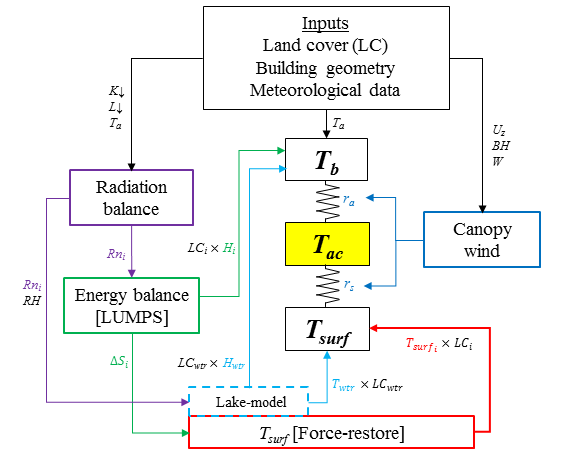
\includegraphics[scale=1.0]{images/Overview.png}
 \caption{Overview of approach used in \glssymbol{Toolkit2} microclimate module.} \label{fig:overview}
\end{figure}

\section{Model Overview}\label{sec:ModelOverview}

\subsection{Data inputs}\label{sec:datainputs}
\subsubsection{Land cover}\label{sec:landcover}

The model uses simple data inputs, which are designed to be easily accessible. The model requires the user to define the land cover fractions of building (\glssymbol{Fbldg}), concrete (\glssymbol{Fconc}), asphalt (\glssymbol{Fasph}), grass (\glssymbol{Fgras}), irrigated grass (\glssymbol{Figrs}), tree (\glssymbol{Ftree}), and water (\glssymbol{Fwatr}). These land cover categories are self-explanatory and describe most of the surfaces in urban areas. Low vegetation (shrubs and bushes) can be included in \glssymbol{Ftree} and \glssymbol{Fbldg} collectively refers to all buildings in urban areas.  In addition to the land cover fractions, the model requires average building height (\glssymbol{BH}) and street width (\glssymbol{W}) information. These data are only needed if the user intends to calculate \glssymbol{Tac}­. In future, look up tables for these land cover variables, based on land-use or local-climate zones (LCZ) \citep{Stewart2012a} could be developed. 

\subsubsection{Meteorological data}\label{sec:metdata}

\glssymbol{Toolkit2} requires reference meteorological data to force the model. The model requires the following inputs: incoming shortwave radiation (\glssymbol{kdown}), incoming long wave radiation (\glssymbol{ldown}) (can be modelled if not available, see appendix), relative humidity (\glssymbol{RH}), reference level wind speed (\glssymbol{Uz}), and reference level air temperature (\glssymbol{Ta}).  Reference meteorological should be representative of background meteorological conditions (i.e. not significantly affected by microclimate effects).  We recommend using the nearest BoM airport weather station for reference meteorological data. BoM radiation data from a small selection of sites is freely available online\footnote{There are options available for modelling K↓, such as the Net All-wave Radiation Parameterization (NARP) of \cite{Offerle2003}, which could be integrated if needed.}.  However, other meteorological variables (\glssymbol{Ta}, \glssymbol{RH}, and \glssymbol{Uz}) are not always freely available and may need to be purchased from the BoM for a small fee. Alternatively, the CRCWSC could generate and make available reference meteorology datasets for each of Australian capital city. 

\section{Model description}\label{sec:ModelDescription}
\subsection{Net energy}\label{sec:net}

During daylight hours (\glssymbol{kdown} $\geq$ 10) net radiation (\glssymbol{Rn}) for the ith surface type is calculated using the following \citep{Loridan2011}


\begin{equation} 
\glssymbol{Rn}  
 = \glssymbol{kdown} 
 (1-\glssymbol{albedo}_{i}) +  \glssymbol{epsilon}_{i}(\glssymbol{ldown}-\glssymbol{sigma} \glssymbol{Ta}^{4}) - 0.08\glssymbol{kdown} (1- \glssymbol{albedo}_{i})) 
\label{eq:rn} \end{equation} 


where \glssymbol{albedo}$_{i}$ is \glsdesc{albedo}, \glssymbol{epsilon}$_{i}$ is \glsdesc{epsilon}, \glssymbol{Ta} is forcing air temperature (K), and \glssymbol{sigma} is the \glsdesc{sigma}. The \glssymbol{albedo}$_{i}$ and \glssymbol{epsilon}$_{i}$ values are predefined for each surface (see  Table 2.1 (TODO LABEL), validation report).  The right hand side of the equation accounts for net longwave radiation, and \glssymbol{lup} is approximated using \glssymbol{Ta}. \cite{Loridan2011}. include the term 0.08\glssymbol{kdown}$(1-\glssymbol{albedo}_{i})$ to account for the difference between near surface \glssymbol{Ta} and \glssymbol{Tsurf}. However, currently there is no correction for this difference at night. As such, we substitute Ta for. The modelled \glssymbol{Tsurf} (from 2 time steps (t) previous) is used to calculate L↑ at night. It is necessary to use  due to the method used to calculate the storage heat flux (eq. 5 TODO REFERENCE), which requires \glssymbol{Rn} from the previous time step.  Testing suggests this lag does not significantly affect calculations when a 30 minute time step is used. Thus, at night (\glssymbol{kdown} $<$ 10) net radiation for i surface type is

\begin{equation} 
\glssymbol{Rn}  
 = \glssymbol{kdown} 
 (1-\glssymbol{albedo}_{i}) + \glssymbol{epsilon}_{i}] \big(\glssymbol{ldown}-\glssymbol{sigma} T_{surf[t-2]}^{4} \big) 
\label{eq:rn2} \end{equation} 


The \glssymbol{Rn} for each surface type is then used to calculate a surface energy balance for each surface. 
\subsection{Surface energy balance (LUMPS)}\label{sec:lumps}

The energy balance calculations are based on the Local-scale Urban Meteorological Parameterisation Scheme (LUMPS) \citep{Grimmond2002a}. For non-water surfaces, the sensible (\glssymbol{H}) and latent (\glssymbol{LE}) heat fluxes for the $i$th surface type are calculated using


\begin{equation} 
\glssymbol{H}_{i} = 
\frac{(1-\glssymbol{pm}_{i})+(\frac{\glssymbol{gamma}}{\glssymbol{s}})}{1+\frac{\glssymbol{gamma}}{\glssymbol{s}}}
(R_{n,i} -\Delta S_{i})- \glssymbol{beta}
\label{eq:H} \end{equation} 

\begin{equation} 
\glssymbol{LE}_{i} = 
\frac{\glssymbol{pm}_{i}}{1+\frac{\glssymbol{gamma}}{\glssymbol{s}}}
(R_{n,i}-\Delta S_{i})+ \glssymbol{beta}
\label{eq:LE} \end{equation} 

where \glssymbol{s} is the slope of the saturation vapour pressure–versus-temperature curve, \glssymbol{gamma} is the psychrometric constant and \glssymbol{pm}$_{i}$ and \glssymbol{beta} are based on a simplification of the Penman–Monteith approach, which takes into account the Priestley–Taylor coefficient; \glssymbol{pm}$_{i}$ depends on the surface moisture status, and \glssymbol{beta} is an empirical constant, set to 3 W m$^{-2}$ \citep{Grimmond2002a}. By default, the \glssymbol{pm} parameter is set using values from \cite{Hanna1992} (Table A1 TODO REFERENCE). Alternatively, \glssymbol{pm} for vegetated classes can be defined as a function of stomatal resistance (sr) using $\glssymbol{pm} = 6.9\times10^{-6} sr^{2} - 0.004 sr + 1.3$ \citep{DeBruin1983}.  

The objective hysteresis model (OHM) is used to calculate storage heat flux for the $i$th land cover class  \citep{Grimmond2002a} 

\begin{equation} 
\Delta S_{i} = R_{n,i} a_{1,i} + \Big( \frac{\partial R_{n,i}}{\partial t}   \Big)a_{2,i} + a_{3,i}
\label{eq:ohm} \end{equation} 


where the three coefficients \glssymbol{a1}, \glssymbol{a2}, and \glssymbol{a3}, are defined for each surface (see examples in Table 2.1 TODO REFERENCE - validation report), and $\frac{\partial R_{n,i}}{\partial t} =0.5(R_{n,it-1} - R_{n,it+1})$  .  The $\Delta S_{i}$ is then used to calculate the surface temperature using the `force-restore' method.


\subsection{Surface temperature calculation (`force-restore')}\label{sec:tsurf}

The change in surface temperature \glssymbol{Tsurf} for surface $i$ with respect to time (t) is calculated as

\begin{equation} 
\frac{\partial T_{surf,i}}{\partial t}= \frac{\Delta S_{i}}{C_{i} D} - \frac{2 \pi}{\tau} (T_{surf,i -1} - T_{m,it-1})
\label{eq:tsurf} \end{equation} 

Where $C_{i}$ is the \glsdesc{C}, $\tau$ is the period (86400 seconds), $D = 2 \glssymbol{kappa} _{i}  / \omega 0.5$, $\glssymbol{kappa} _{i}$ is the \glsdesc{kappa}, and $\glssymbol{kappa} = 2\pi / \tau$.  The first term on the right-hand side is the forcing term that affects \glssymbol{Tsurf}, while the second term is the restore term which dampens the forcing term. The \glsdesc{Tm} ($T_{m,i}$) is calculated using

\begin{equation} 
\frac{\partial T_{m,i}}{\partial t} = \frac{\Delta S_{i}}{C_{i} D_{y}}
\label{eq:tm} \end{equation} 

where \glssymbol{Dy} = $D \sqrt{365}$, the \glsdesc{Dy}. 

Thus for each time step, the aggregated \glssymbol{Tsurf} and \glssymbol{H} are equal to

\begin{equation} 
\glssymbol{H} = \sum_{i=1}^{6} (F_{i} H_{i}) + (F_{wtr} H_{wtr})
\label{eq:H} \end{equation} 

\begin{equation} 
\glssymbol{Tsurf} = \sum_{i=1}^{6} (F_{i} T_{surf,i}) + (F_{wtr} T_{wtr})
\label{eq:tsurf} \end{equation} 

As the force-restore method cannot be applied to water, we use a simple a simple water body model to calculate $H_{wtr}$ and $T_{wtr}$.
%
%3.4 Simple water body model 
%
%The water model in the toolkit is based on a single water layer, overlaying a soil layer. Essentially, the force-restore surface temperature model is implemented, and is overlain by a homogeneous mixed water layer (i.e. neglecting thermal stratification) representing a water body of depth z (m). The model is designed to apply to water bodies of 0.1 – 1.0 m depths. The water model is based on the pan evaporation model of Martinez et al. (2006) which closely follows that of the lake model of Jacobs et al. (1997). The water body model also determines the surface energy balance of the water surface. The energy balance model for the water layer is given by (Martinez et al., 2006):
%
%			(eq. 10)
%
%where Sab is absorbed shortwave radiation, L* the net longwave, Gwtr is the convective heat flux at the bottom of the water layer (and into the soil below), and ΔSwtr is the change in heat storage of the water layer. Solar radiation penetrates the water surface and is absorbed as described by Beer’s Law (Martinez et al., 2006):
%
%				(eq. 11)
%
%where K* is the net shortwave radiation, \glssymbol{beta}K is the amount of shortwave radiation immediately absorbed by the water layer (set to 0.45) (Martinez et al., 2006), and η the extinction coefficient. Here, η is given the following from Subin et al. (2012), for the water layer with depth z (m):
%
%						(eq. 12)
%A correction factor for the solar path length zenith angle is often applied to Eq. 11 (Martinez et al., 2006) but this has been omitted to reduce complexity. The convective heat transport Gwtr into the soil at the base of the water layer is given by (Martinez et al., 2006):
%
%						(eq. 13)
%where Cwtr is the volumetric heat capacity of water (4.18×106 J m-3 K-1), κwtr is the eddy diffusivity pf water (m2 s-1), and the change in depth Δz = z (the depth of the water layer), the change in temperature ΔT (°C) is the difference between the water temperature  (°C) and the soil temperature Ts (°C). These initial temperatures ( & Ts) must be specified (at time t = 0, they can be set to the same value). κwtr is a complex function accounting for thermal stratification and surface friction velocity. Again, to reduce complexity and assuming a mixed homogeneous water layer, a constant κwtr has been selected based on shallow lakes reported in Salas de Leon et al. (2016) (Table A2).
%
%The latent heat flux (LEwtr) (W m-2) is given by (Arya, 2001):
%
%						(eq. 14)
%
%where ρv is the density of moist air (kg m-3), Lv is the latent heat of vaporisation (set to 2.43 MJ kg-1) hv is the bulk transfer coefficient for moisture (1.4 × 10-3; Jones et al., 2005; Hicks, 1972), Uz the BoM reference wind speed, qs the saturated specific humidity at Twtr, and qa is the specific humidity of the air at Ta (see appendix for calculation of ρv qs and qa). The sensible heat flux is given by Martinez et al. (2006)2:
%
%						(eq. 15) 
%
%where ρa is the density of dry air (1.2 kg m-3), cp the specific heat of air (1013 J kg-1 K-1) and hc the bulk transfer coefficient for heat (hc = hv). Returning to Eq. 11, net long wave radiation L* = \glssymbol{Rn} - K* leaving ΔSwtr from the energy balance equation, which is defined as (Martinez et al., 2006):
%
%							(eq. 16)
%
%where Δt is change in time (seconds) and Cwtr is the volumetric heat capacity of water.. Solving for ΔTwtr and adding the change in temperature to the previous time step (Twtr = Twtr [t-1) + ΔTwtr) gives the new water layer temperature. 
%
%Below the water layer, the Force-Restore model (Eq. 6) determines the soil surface temperature where Gwtr is equivalent to   for other surfaces. The soil layer parameters are set to saturated soil where the volumetric heat capacity is set to C = 3.03 × 106 (J m-2 K-1) and the thermal diffusivity is set to κ = 0.625 × 10-6 (m2 s-1). 
%
%
%
%3.5 Calculation of urban canopy layer air temperature (Tac) 
%
%The Tac term is calculated following the approach outlined in Figure 1.2. 
%
%
%Figure 1.2: Schematic of the air temperature module
%
%First we, solve the following equation for Tb (Yang et al 2011). This assumes a generic local scale Ta for the site (all grid cells). 
%					(eq. 17)
%
%where cp is the specific heat of air (1013 J kg-1 K-1) and ρa is the density of air (1.2 kg m-3). 
%The canopy to atmosphere resistance (ra) is given by (Yang et al 2011):
%
%					(eq. 18)
%
%Where zu is BoM measurement height, d is zero plane displacement height (2/3 height of roughness elements), z0 is roughness length (0.1 x height of roughness elements). 
%
%The temperature of the canopy layer (Tac) is then given by (Oelson et al., 2010):
%
%					(eq. 19)
%
%which is a simplification of Equation 3.75 (appendix) in the CLMU technical note (Oelson et al., 2010):, because we do not consider sensible heat conductance for individual surface types. Sensible heat conductance are given for the urban canopy layer to atmosphere (Hca) and surface to urban canopy layer (Hcs) by (Oelson et al., 2010):
%				(eq. 20)	
%
%where rs is the surface to urban canopy resistance (s m-1):
%
% 				(eq. 21)
%Ucan is the canyon wind speed:
%				(eq. 22)
%
%where Utop is the wind speed at the top of the canopy layer (m s-1), BH is the building height (m) and W is the street width (m). Utop is estimated at the top of the UCL based on Uz using a logarithmic relationship:
%
%  				(eq. 23)
%
%If BH is below the domain average building height, it should be set to the domain average. 

\printglossary[title={List of Symbols}]

\section{Code availability}\label{sec:available}



\section*{Acknowledgements}
The support of the Commonwealth of Australia through the Cooperative Research Centre program is acknowledged.
%\end{acknowledgements}

\section*{References}\label{sec:ref}
%% If you have bibdatabase file and want bibtex to generate the
%% bibitems, please use
%%
  \bibliographystyle{elsarticle-harv} 
  \bibliography{library}

%% else use the following coding to input the bibitems directly in the
%% TeX file.

\begin{thebibliography}{00}

%% \bibitem[Author(year)]{label}
%% Text of bibliographic item

\bibitem[ ()]{}

\end{thebibliography}


%% The Appendices part is started with the command \appendix;
%% appendix sections are then done as normal sections
\appendix
\setcounter{table}{0}
\renewcommand{\thetable}{A\arabic{table}}

%\subsection{}                               %% Appendix A1, A2, etc.


%%%%%%%%%% taking out parameterizations
\section{MAESPA vegetation parameterisations}\label{sec:maespavegpara}  
%
%Appendix
%
%Table A1: Previously quoted values for pm: range listed by Hanna and Chang (1992) based on information presented by Beljaars and Holtslag (1989, 1991). 
%Surface type
%pm
%Dry desert with no rain for months
%0.0 - 0.2
%Arid rural area
%0.2 - 0.4
%Crops and field, midsummer (minimal rain)
%0.4 - 0.6
%Urban environment, some parks
%0.5 - 1.0
%Crops, fields, or forest with sufficient soil moisture
%0.8 - 1.2
%Large lake or ocean
%1.2 - 1.4
%
%
%Table A2. Selected values of eddy diffusivity for shallow lakes (Salas de Leon et al., 2016).
%Location
%z (m)
%Kw (m2 s-1)
%Source
%El Porcal, Spain
%6
%13.0 × 10-7
%Álvarez-Cobelas et al. (1986)
%Mendota, USA
%12
%1.4 × 10-7
%Dutton and Bryson (1962)
%Linsley Pond, USA
%6.5
%3.3 × 10-7
%Hutchinson (1957)
%Sodom, USA
%7.6
%7.0 × 10-7
%Hutchinson (1957)
%Average
%8.0
%6.18 × 10-7
%
% 
%Equation 3.75 from CLMU tech note.
%
%
%Ancillary calculations
%
%Calculation of saturation vapour pressure (es) (kPa) at the water surface:
%
%
%Calculation of vapour pressure (kPa) of the air (ea):
%
%
%Calculation of saturated specific humidity (qs) (kg kg-1) at the water surface, where P is the pressure (101.3 kPa) 
%		
%
%Calculation of the specific humidity of air (qa), 
%
%
%Calculation of density of moist air (ρv) (kg m-3)
%
%
%If L↓ data are not available, \glssymbol{Toolkit2} contains a built-in function to model L↓ using (Loridan et al., 2010):
%
%where the clear sky emissivity and FCLD­ is the cloud cover fraction at measurement time. 
%
%
%where 
%% % % % % % % % % % % % % % % % % % % % % % % %


%\authorcontribution{This work was developed by Kerry Nice and supervised by Andrew Coutts and Nigel Tapper. Model source code was received from Scott Krayenhoff and Remko Duursma (as acknowledged in Section \ref{sec:available}). Synthesis of this code and new code was developed by Kerry Nice. The article was written by Kerry Nice with editing and suggestions from Andrew Coutts and Nigel Tapper.}
%
%\begin{acknowledgements}
%The work described in this paper was developed during a PhD. project at Monash University. Funding for this was obtailed through the City of Melbourne, Monash University, and the CRC for Water Sensitive Cities.  
%\end{acknowledgements}

%\begin{acknowledgements}
%The support of the Commonwealth of Australia through the Cooperative Research Centre program is acknowledged.
%\end{acknowledgements}

%%%% \section{}
%%%% \label{}
%%\section{References}\label{sec:ref}
%%%% If you have bibdatabase file and want bibtex to generate the
%%%% bibitems, please use
%%%%
%%  \bibliographystyle{elsarticle-harv} 
%%  \bibliography{library}
%%
%%%% else use the following coding to input the bibitems directly in the
%%%% TeX file.
%%
%%\begin{thebibliography}{00}
%%
%%%% \bibitem[Author(year)]{label}
%%%% Text of bibliographic item
%%
%%\bibitem[ ()]{}
%%
%%\end{thebibliography}
%%
%%
%%
%%
%%



\end{document}

\endinput
%%
%% End of file `elsarticle-template-harv.tex'.
